\section{El problema}

% Escala de color de la sección (bloques del tema):
%   exampleblock (olivo) → contexto · block (verde) → desarrollo · alertblock (terracota) → punto crítico

% ── Frame: Tres bloques ───────────────────────────────────────────────────────
\begin{frame}{Un problema político que se volvió estructural}
  \begin{columns}[T]
    \begin{column}{0.32\textwidth}
      \begin{exampleblock}{\parbox[c][2.2em][c]{\linewidth}{\small Centralización\\del poder}}
        \begin{minipage}[t][2.8cm][t]{\linewidth}\small
          La capital concentra la toma de decisiones políticas,
          estructurales, sociales y económicas: \textbf{CDMX $\neq$ EDOMEX}.
        \end{minipage}
      \end{exampleblock}
    \end{column}
    \begin{column}{0.32\textwidth}
      \begin{block}{\parbox[c][2.2em][c]{\linewidth}{\small Feudos de\\transporte}}
        \begin{minipage}[t][2.8cm][t]{\linewidth}\small
          Aunque existen diferentes medios de transporte público, cada uno tiene su propio sindicato y particularidades.
        \end{minipage}
      \end{block}
    \end{column}
    \begin{column}{0.32\textwidth}
      \begin{alertblock}{\parbox[c][2.2em][c]{\linewidth}{\small Eres libre de pensar,\\no de actuar}}
        \begin{minipage}[t][2.8cm][t]{\linewidth}\small
          Existen los datos, existen los intereses, pero se necesita una combinación de circunstancias para lograrlo.
        \end{minipage}
      \end{alertblock}
    \end{column}
  \end{columns}
\end{frame}

% ── Frame: Centralidad de la CDMX ────────────────────────────────────────────
\begin{frame}{CDMX: El centro del poder político y económico}
  \begin{columns}[T]
    \begin{column}{0.54\textwidth}
      \small
      \begin{itemize}
        \item La \zmvm\ es una de las urbes más antiguas del continente americano. Siendo fundada en 1325
        bajo el mandato del emperador Mexica Tenoch, con el nombre de Tenochtitlan (lugar de tunas) \citep{molina2013erase}.
        % \pause
        \item La ZMVM se constituye como una \termino{región nodal} donde la Ciudad de México actúa como centro articulador de
              un sistema complejo de flujos, servicios y desigualdades socio-espaciales.
      \end{itemize}
    \end{column}
    \begin{column}{0.44\textwidth}
      \begin{block}{Dato clave}
        \footnotesize
        El nombre oficial de México es Estados Unidos Mexicanos, siendo un gobierno Federal donde cada estado tiene su propia autonomía.
        En la práctica esta es una invitación para destinar los recursos públicos del PIB nacional a las zonas de mayor interés; siendo las
        zonas urbanas y metropolitanas las más beneficiadas (ZMVM, ZMGDL, ZMNL), mientras que las zonas rurales y periféricas quedan relegadas.
      \end{block}
    \end{column}
  \end{columns}
\end{frame}

% ── Frame: Modelos de estructura urbana ──────────────────────────────────────
\begin{frame}{Modelos de Estructura Urbana en la ZMVM}
  \begin{columns}[c]
    % --- COLUMNA IZQUIERDA: EXPLICACIÓN COMPLEMENTARIA ---
    \begin{column}{0.55\textwidth}
      \footnotesize
      \vspace*{-0.3cm}
      \begin{itemize}\setlength{\itemsep}{0.05cm}
        \item \textbf{Anillos:} Crecimiento radial desde el núcleo central hacia periferias residenciales.
        \item \textbf{Sectores:} Formación de cuñas siguiendo ejes de transporte; ej. Corredor
              \textit{Reforma-Santa Fe} (lujo) e \textit{Industrial Vallejo} (norte).
        \item \textbf{Núcleos:} La CDMX como múltiples polos independientes como
              \textit{Satélite, Polanco, CU y Santa Fe} \citep{padilla2022expansion}.
      \end{itemize}
      \vspace{-0.15cm}

      \begin{exampleblock}{\footnotesize Análisis Topológico}
        \scriptsize Según \citet{jia2010}, pueden distinguirse tres patrones espaciales de
        desarrollo urbano: el desarrollo saltón muestra mayor fragmentación y
        aislamiento; el lineal implica menor fragmentación pero mayor aislamiento; y el
        compacto, aunque más eficiente, también puede derivar en expansión si la
        densidad residencial disminuye (traducción propia).
      \end{exampleblock}
    \end{column}
    \begin{column}{0.43\textwidth}
      \centering
      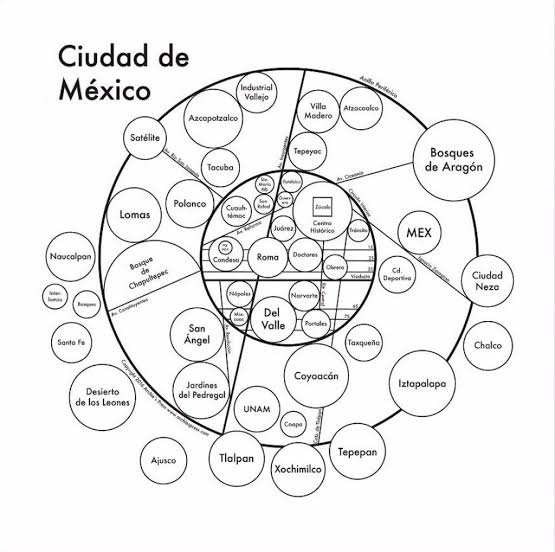
\includegraphics[width=\textwidth, height=0.62\textheight, keepaspectratio]{ArichieExpress.JPEG}

      {\scriptsize Esquema de nodos y flujos.}
      \fuentefigura{Archie's Press.}
    \end{column}
  \end{columns}
\end{frame}

% ── Frame: Tres imágenes con texto explicativo ────────────────────────────────
\begin{frame}{Modelo de Expansión}
  \begin{columns}[T]
    \begin{column}{0.32\textwidth}
      \centering
      \begin{exampleblock}{\scriptsize Fase 1: Nodo en expansión}
        \centering
        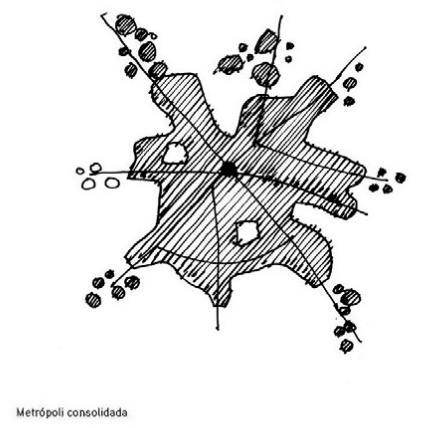
\includegraphics[width=\textwidth, height=2.8cm, keepaspectratio]{dispersion_diagrama_3.png}

        \begin{minipage}[t][1.5cm][t]{\linewidth}\scriptsize
          La ciudad contiene áreas periféricas definidas, pero estas no son nodos, sino
          extensiones del centro.
        \end{minipage}
      \end{exampleblock}
      \fuentefigura{\citet{padilla2022expansion}.}
    \end{column}

    \begin{column}{0.32\textwidth}
      \centering
      \begin{block}{\scriptsize Fase 2: Nodo en conexión}
        \centering
        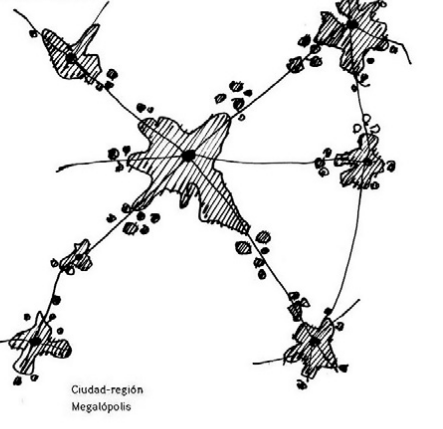
\includegraphics[width=\textwidth, height=2.8cm, keepaspectratio]{dispersion_diagrama_4.png}

        \begin{minipage}[t][1.5cm][t]{\linewidth}\scriptsize
          Los nodos toman fuerza y crean conexiones visibles desde sus centros hacia sus periferias.
        \end{minipage}
      \end{block}
      \fuentefigura{\citet{padilla2022expansion}.}
    \end{column}

    \begin{column}{0.32\textwidth}
      \centering
      \begin{alertblock}{\scriptsize Fase 3: Consolidación}
        \centering
        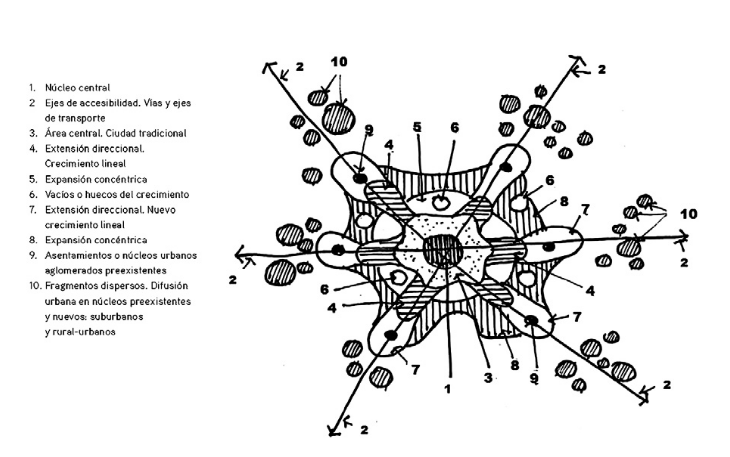
\includegraphics[width=\textwidth, height=2.8cm, keepaspectratio]{dispersion_diagrama_1.png}

        \begin{minipage}[t][1.5cm][t]{\linewidth}\scriptsize
          La región se consolida como una megalópolis con un nodo central y nodos satélites
          conectados por diferentes aristas articuladoras.
        \end{minipage}
      \end{alertblock}
      \fuentefigura{\citet{padilla2022expansion}.}
    \end{column}
  \end{columns}
\end{frame}
